\documentclass[12pt, a4paper]{article}

\usepackage{VUMIFCS1magistrinis}
\usepackage{cite}
\usepackage{amsmath}
\usepackage{bm}
\usepackage{amsfonts}
\usepackage{float}
\usepackage{graphicx}
\usepackage{color}
\usepackage{listings}
\usepackage{wrapfig}
\usepackage{algpseudocode}
\usepackage{algorithm}
\usepackage{algorithmicx}
\usepackage{caption}
\usepackage{subfig}


% Titulinio aprašas
\university{Vilniaus universitetas}
\faculty{Matematikos ir informatikos fakultetas}
\vumifdept{Informatikos katedra}
\vumifpaper{Magistro baigiamasis darbas}
\title{Rizikų valdymo proceso modeliavimas}
\titleineng{Modeling of Risk Management Process}
\status{2 kurso 1 grupės studentas}
\author{Vardenis Pavardenis}
% \secondauthor{Vardonis Pavardonis}
\supervisor{prof. habil. dr. Vardaitis Pavardaitis}
\reviewer{doc. dr. Vardauskas Pavardauskas}
\date{Vilnius – \the\year}

\begin{document}
\maketitle

%% Padėkų skyrius
% \sectionnonumnocontent{}
% \vspace{7cm}
% \begin{center}
%     Padėkos asmenims ir/ar organizacijoms
% \end{center}

\sectionnonumnocontent{Santrauka}
Glaustai aprašomas darbo turinys, pristatoma nagrinėta problema ir padarytos
išvados. Santraukos apimtis ne didesnė nei 0,5 puslapio. Santraukų gale
nurodomi darbo raktiniai žodžiai. 
% Nurodomi iki 5 svarbiausių temos raktinių žodžių (terminų).
% Vienas terminas gali susidėti iš kelių žodžių.
\raktiniaizodziai{raktinis žodis 1, raktinis žodis 2, raktinis žodis 3, raktinis žodis 4, raktinis žodis 5}   

\sectionnonumnocontent{Summary}
Santrauka anglų kalba.
\keywords{keyword 1, keyword 2, keyword 3, keyword 4, keyword 5}

\tableofcontents

\sectionnonum{Įvadas}
Įvade aprašomi darbo tikslai, nurodomas temos aktualumas, aptariamos teorinės
darbo prielaidos bei metodologija, apibrėžiamas tiriamasis objektas,
apibūdinami su tema susiję literatūros ar kitokie šaltiniai, temos analizės
tvarka, darbo atlikimo aplinkybės, pateikiama žinių apie naudojamus
instrumentus (programas ir kt.). Rekomenduojama įvado apimtis 3-4 puslapiai.

\section{Medžiagos darbo tema dėstymo skyriai}
Medžiagos darbo tema dėstymo skyriuose pateikiamos nagrinėjamos temos detalės:
pradiniai duomenys, analizės ir apdorojimo metodai, sprendimų įgyvendinimas,
gautų rezultatų apibendrinimas.

\subsection{Poskyris}
Citavimo pavyzdys \cite{Banerjee1997}, \cite{EgArticle}.
% "`, "' - Lietuviškos kabutės 
\subsubsection{Skirsnis}
\subsubsubsection{Straipsnis}
\subsubsection{Skirsnis}
\section{Skyrius}
\subsection{Poskyris}
\subsection{Poskyris}

\sectionnonum{Rezultatai ir išvados}
Rezultatų ir išvadų dalyje išdėstomi pagrindiniai darbo rezultatai (kažkas
išanalizuota, kažkas sukurta, kažkas įdiegta), pateikiamos išvados (daromi
nagrinėtų problemų sprendimo metodų palyginimai, siūlomos rekomendacijos,
akcentuojamos naujovės).

\bibliography{bibliografija}   % Literatūros šaltiniai aprašomi bibliografija.bib faile
% Šaltinių sąraše nurodoma panaudota literatūra, kitokie šaltiniai. Abėcėlės
% tvarka išdėstoma tik darbe panaudotų (cituotų, perfrazuotų ar bent paminėtų)
% mokslo leidinių, kitokių publikacijų bibliografiniai aprašai (šiuo punktu
% pasirūpina LaTeX). Aprašai pateikiami netransliteruoti.

\sectionnonum{Santrumpos}
Sąvokų apibrėžimai ir santrumpų sąrašas sudaromas tada, kai darbo tekste
vartojami specialūs terminai, reikalaujantys paaiškinimo, ir rečiau sutinkamos
santrumpos.

\appendix  % Priedai
% Prieduose gali būti pateikiama pagalbinė, ypač darbo autoriaus savarankiškai
% parengta, medžiaga. Savarankiški priedai gali būti pateikiami kompiuterio
% diskelyje ar kompaktiniame diske. Priedai taip pat vadinami ir numeruojami.
% Tekstas su priedais siejamas nuorodomis.

\section{Niauroninio tinklo struktūra}
\begin{figure}[H]
    \centering
    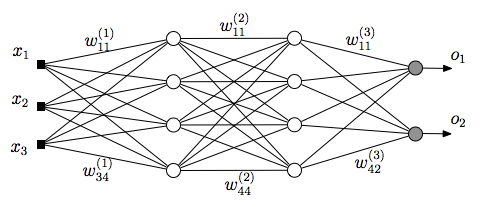
\includegraphics[scale=0.5]{img/MLP}
    \caption{Paveikslėlio pavyzdys}
    \label{img:mlp}
\end{figure}


\section{Eksperimentinio palyginimo rezultatai}
% tablesgenerator.com - converts calculators, e.g. excel, tables to LaTeX
\begin{table}[H]\footnotesize
  \centering
  \caption{Lentelės pavyzdys.}
  {\begin{tabular}{|l|c|c|} \hline
    Algoritmas & $\bar{x}$ & $\sigma^{2}$ \\
    \hline
    Algoritmas A  & 1.6335    & 0.5584       \\
    Algoritmas B  & 1.7395    & 0.5647       \\
    \hline
  \end{tabular}}
  \label{tab:table example}
\end{table}

\end{document}
